% Compile this file in Overleaf using the official IEEEtran class.
\documentclass[conference]{IEEEtran}
\usepackage[T1]{fontenc}
\usepackage{graphicx,booktabs,array,microtype}
\usepackage[hidelinks]{hyperref}
\graphicspath{{figures_d3/}{interface_v2/}}
\title{Temporal Robustness of Graph and Tabular Models for Illicit Bitcoin Transaction Detection}
\author{\IEEEauthorblockN{Alex (GitHub: alexchooys)}
\IEEEauthorblockA{Applied Data Science, University of Florida\\\url{https://github.com/alexchooys}}}
\begin{document}\maketitle
\begin{abstract}
This refinement study extends an Elliptic transaction-classification prototype from one seed to three while preserving its temporal protocol. XGBoost, a multilayer perceptron (MLP), and GraphSAGE are evaluated under frozen, expanding-history, rolling-window, and recency-weighted policies. Recomputed metrics agree with 600,120 saved prediction records across 540 model--policy--seed--snapshot results. Recency-weighted XGBoost retains mean post-shift average precision (AP) 0.4053. Corresponding three-seed results are $0.1303\pm0.0355$ for MLP and $0.1077\pm0.0459$ for GraphSAGE, where dispersion denotes sample standard deviation across runs. No combination meets the support-aware sustained-recovery criterion by snapshot 49. Incoming-degree diagnostics reveal sparse illicit support in connected subgroups and no consistent graph-model advantage. Interface refinements add seed comparisons, explicit threshold decisions, validated CSV prediction, and queue export. A paired Colab benchmark reduces median warm callback latency from 55.19 to 18.60 ms while preserving metrics and queue IDs. Results support a stronger reliability assessment and a more usable prototype, rather than a claim of new independent test data or uniformly better model accuracy.
\end{abstract}
\noindent\textit{Index Terms---}anti-money laundering, GraphSAGE, temporal adaptation, reproducibility, human review.

\section{Project Summary}
Financial-crime investigators face changing transaction patterns and limited review capacity. This project asks whether graph models and local-feature models respond differently to distribution shift, and whether recent-data adaptation helps one family more than another. The original Elliptic study already examined graph and tree models and documented a performance break around time step 43 \cite{elliptic}. The contribution here is the crossed model--adaptation comparison, supported by controlled temporal evaluation and an interactive research interface.

Deliverable 2 implemented XGBoost, an MLP, and GraphSAGE for seed 0. Deliverable 3 adds seeds 1 and 2, explicit preprocessing records, prediction-level audits, incoming-degree error analysis, and interface improvements. Expanding-history retraining remains the control for receiving more historical labels. The MLP remains essential for distinguishing a neural-model comparison from a graph-information comparison.

The refinements address reliability and usability rather than expanding the architecture search. They show which conclusions persist across initialization and validation selection, expose threshold behavior that AP alone hides, and reduce input and inspection effort. The original seed-0 experiment is retained unchanged. The extended estimate includes that run; it is not an independent replication on new transactions. New training, degree analysis, native inference verification, and a runtime benchmark have executed in Colab. Browser captures document the revised comparison, explorer, and input screens. An independent human usability study has not been conducted.

\section{Updated System Architecture and Pipeline}
\subsection{Data and Temporal Boundaries}
The original Elliptic release contains 203,769 transaction nodes, 234,355 directed edges, and 49 snapshots. Labels comprise 4,545 illicit, 42,019 licit, and 157,205 unknown transactions. Unknown targets remain masked rather than treated as legitimate. The predictor set remains 93 local numerical attributes; transaction ID, time, labels, and the 72 supplied neighborhood aggregates are excluded. These choices preserve comparability with Deliverable 2.

Training uses steps 1--30, validation uses 31--34, and testing uses 35--49. The respective known-label counts are 26,905, 2,989, and 16,670, including 2,954, 508, and 1,083 illicit targets. Step 32 contributes 342 validation illicit labels, so threshold selection remains concentrated in one snapshot. Checks verify finite values, unique IDs, feature order, graph endpoints, and zero cross-time edges. The feature schema and split counts are saved as reusable artifacts.

\begin{figure*}[t]\centering
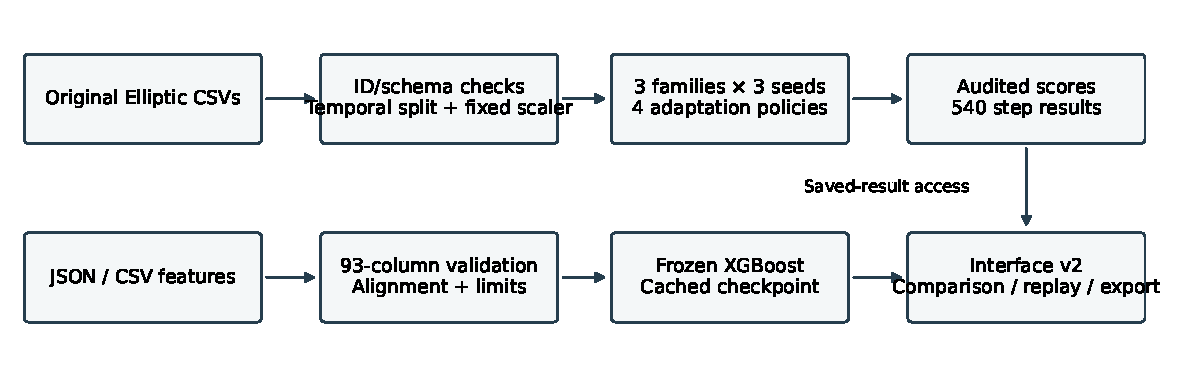
\includegraphics[width=0.96\textwidth]{architecture_v2.pdf}
\caption{Refined architecture. Offline training produces audited artifacts for comparison and replay. A separate validated input path serves the frozen XGBoost checkpoint. Interface controls never initiate retraining.}\label{fig:architecture}\end{figure*}

Neural inputs use a standard scaler fitted only on labeled initial-training nodes and held fixed. XGBoost receives the original released feature values without that scaler. GraphSAGE retains unknown nodes as feature/edge context but excludes their targets from loss. Training and validation graphs contain 123,287/12,978 nodes and 142,784/14,059 edges, respectively. Scoring graphs contain only their own snapshot; the absence of cross-time edges supports this separation. Retrospective snapshot access is still an assumption, not proof of real-time availability.

\subsection{Models and Adaptation}
XGBoost \cite{xgboost} uses 150 trees, depth 4, learning rate 0.05, and histogram construction. The MLP has layers $93\rightarrow64\rightarrow64\rightarrow1$, ReLU, dropout 0.2, and 10,241 parameters. GraphSAGE \cite{sage} uses two 64-unit mean-aggregation layers and a linear output, with 20,289 parameters. Original incoming directed edges are preserved. Both neural models use Adam with learning rate 0.001 and weight decay $10^{-4}$.

Initial neural training allows 200 epochs with patience 25 on validation AP and a minimum improvement of $10^{-5}$. Checkpoints and thresholds are selected separately for each seed. Thresholds maximize validation F1 on the 0.05--0.95 grid, favoring the larger threshold on ties. The initial negative-to-positive ratio, 8.107989, remains the fixed positive-class weight. No test outcomes select these settings.

For prediction at step $t$, adaptive models refit from scratch using known labels from steps strictly earlier than $t$. Expanding uses all permitted history. Rolling uses the previous eight snapshots. Recency weights a historical step $s$ by $2^{-((t-1)-s)/4}$ and normalizes weights to mean one. Weighted neural losses divide by the sum of sample weights. Adaptive neural refits use the seed's selected epoch budget without test-based early stopping. The one-step label delay is simulated; actual investigation turnaround is unavailable. At step 35, adaptive histories can include validation labels through 34, so the key comparison is recency versus expanding, not an unqualified frozen-to-adaptive gain.

\section{Refinements Since Deliverable 2}
\subsection{Preprocessing and Run Reproducibility}
The new preprocessing cell saves ordered predictor names, excluded columns, label mapping, temporal boundaries, and cross-time checks. It explicitly confirms the verified split sizes. Graph construction maps transaction IDs to tensor positions and checks that sample weights align with labeled node order. New outputs use a dedicated Deliverable 3 directory, while guards prevent accidental replacement of completed seed runs.

\begin{table}[t]\caption{Validation-selected neural settings by seed.}\centering\small
\begin{tabular}{lrrrr}\toprule
Model & Seed & Epoch & Val. AP & Threshold\\\midrule
MLP & 0 & 145 & .8800 & .80\\
MLP & 1 & 200 & .8840 & .80\\
MLP & 2 & 101 & .8706 & .70\\
GraphSAGE & 0 & 73 & .8164 & .85\\
GraphSAGE & 1 & 199 & .8935 & .90\\
GraphSAGE & 2 & 60 & .7989 & .85\\\bottomrule
\end{tabular}\label{tab:settings}\end{table}

Table~\ref{tab:settings} makes selection variability visible. MLP seed 1 reaches the 200-epoch limit; GraphSAGE seed 1 selects epoch 199 from a 200-epoch run. These caps are retained rather than selectively extended. Variation across seeds therefore includes initialization and validation-selected training duration and thresholds. It should not be attributed solely to initialization or graph structure. XGBoost selects threshold 0.70 and validation AP 0.9634 for each seed.

The audit reconstructs AP, precision, recall, F1, confusion counts, and review-budget metrics from saved predictions. It confirms the same test IDs and targets across all combinations and agreement with stored metrics. There are 540 snapshot results from 36 model--policy--seed combinations and 600,120 prediction records. These records repeatedly score the same 16,670 known-label test transactions; they do not represent 600,120 independent examples. The uploaded 85-cell training notebook contains no saved errors. A separate training-only extract avoids rerunning its historical Deliverable 2 section.

\subsection{Caching and Input Validation}
The revised service caches immutable prediction files, metric tables, validation settings, and the live checkpoint. It avoids repeated CSV parsing and model loading during interaction. Cached and original callbacks produce matching selected metrics and queue IDs for the benchmark workload. The app must restart after replacing cached artifacts.

CSV input accepts 1--200 rows with exactly the 93 named local-feature columns. Columns align by name, and missing, duplicate, extra, nonnumeric, nonfinite, and oversized inputs produce explanatory errors. Single-transaction JSON input checks length and numeric type, including rejection of nulls and booleans. Batch input is processed in memory without application-level file persistence. The native XGBoost engine is preferred; a restricted numeric-tree evaluator supports the provided checkpoint when the native library is absent.

\section{Interface Usability and Improvements}
\subsection{Interaction Flow}
The comparison tab places Deliverable 2 seed-0 AP alongside the three-seed mean and sample standard deviation. A separate paired-gain table contrasts recency with expanding history. Both views explain that additional seeds measure run variation and do not provide new independent test periods.

\begin{figure*}[t]\centering
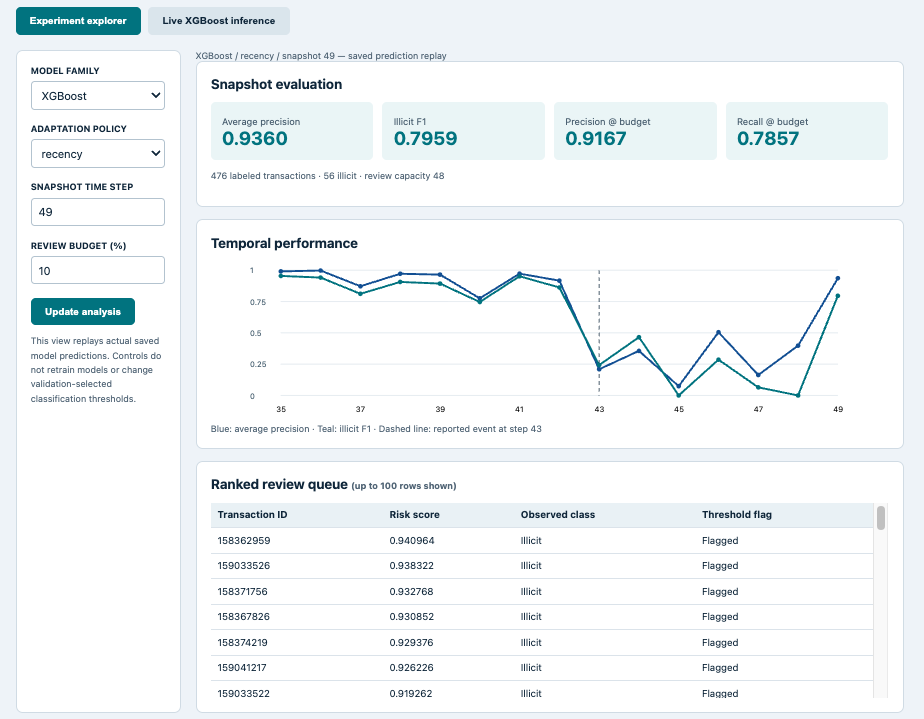
\includegraphics[width=0.485\textwidth]{interface_explorer.png}\hfill
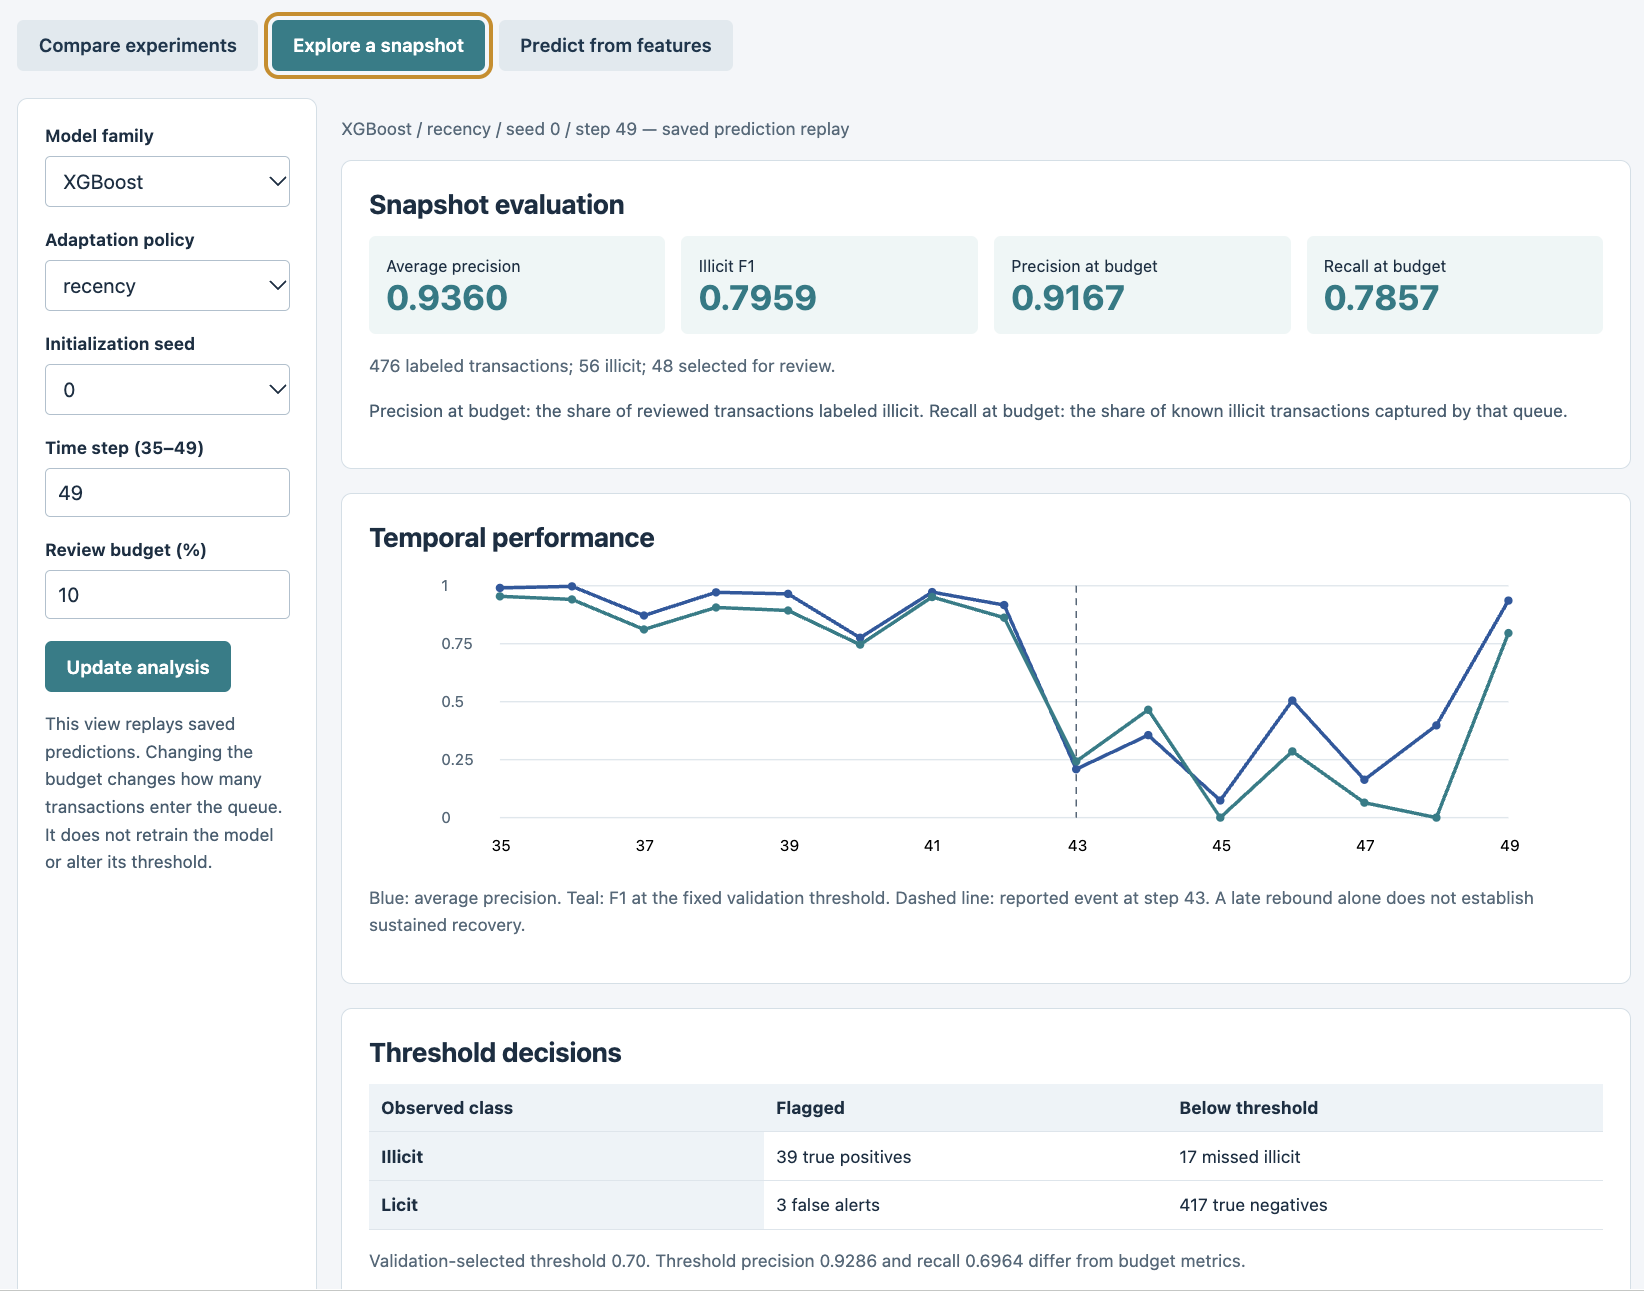
\includegraphics[width=0.485\textwidth]{explorer.png}
\caption{Actual explorer captures. Left: Deliverable 2. Right: Deliverable 3 adds seed selection, clearer budget definitions, and threshold confusion counts. Both show XGBoost/recency/seed 0 at step 49, preserving the same results while improving interpretation.}\label{fig:ui}\end{figure*}

The explorer adds seed selection and threshold confusion counts to the model, policy, snapshot, and review-budget controls. Changing the budget selects a different queue size without altering the validation threshold. The queue export contains the full selected queue, even when the browser limits the displayed rows. Low illicit support triggers a warning. Figure~\ref{fig:ui} compares genuine interface captures rather than a mockup.

The live tab reduces manual entry through a verified real-example button and a downloadable feature CSV. Users can submit one JSON feature array or a validated CSV batch and download batch scores. Live inference remains limited to frozen XGBoost seed 0 at threshold 0.70. Other families and policies support retrospective replay, not live graph inference or adaptive checkpoint serving.

\subsection{Executed Evidence and Usability Limits}
The captured step-49 explorer reports AP 0.9360 and F1 0.7959 for 476 known-label transactions, including 56 illicit. At a 10\% review budget, the top 48 contain 44 illicit transactions: precision 0.9167 and recall 0.7857. The fixed-threshold confusion counts are 39 true positives, 17 false negatives, three false positives, and 417 true negatives. Threshold precision 0.9286 and recall 0.6964 differ from budget metrics because the operating rules select different sets.

A Colab verification checks native inference against saved predictions on 50 actual test rows. Maximum absolute differences are $2.935\times10^{-8}$ for native versus saved and $5.974\times10^{-8}$ for portable versus native, below the $10^{-5}$ absolute/relative tolerance. The app's real example produces native score 0.02013587, below threshold. This confirms model execution for that input, not legitimate activity or representative detection performance. The live-form screenshot shows the layout before prediction; the verification JSON provides the separate executed inference evidence.

Eight backend test methods pass, covering all 540 explorer selections, real-example JSON/CSV consistency, reordered CSV columns, input errors, queue exports, and sparse-support warnings. Browser screenshots confirm rendering and selected interactions. They do not establish every browser download path, mobile responsiveness, accessibility compliance, or independent human usability. A task checklist supports future observation; no participant feedback, satisfaction score, or human task timing is invented.

\section{Extended Evaluation and Updated Results}
\subsection{Primary Metrics and Three-Seed Comparison}
AP denotes average precision, not accuracy or trapezoidal PR-AUC. Primary phase summaries equally average snapshot metrics over steps 35--42 or 44--49, with 43 separate. The three-seed result then averages each seed's phase estimate. Sample SD describes variability between runs and is not a confidence interval for future transaction patterns.

\begin{table}[t]\caption{Recency policy: D2 versus three-seed D3 results.}\centering\small\setlength{\tabcolsep}{3pt}
\begin{tabular}{lccc}\toprule
Model & D2 AP & D3 AP, mean $\pm$ SD & D3 F1\\\midrule
XGBoost & .4053 & $.4053\pm.0000$ & .2685\\
MLP & .1203 & $.1303\pm.0355$ & .0457\\
GraphSAGE & .0817 & $.1077\pm.0459$ & .0083\\\bottomrule
\end{tabular}\label{tab:main}\end{table}

\begin{figure*}[t]\centering
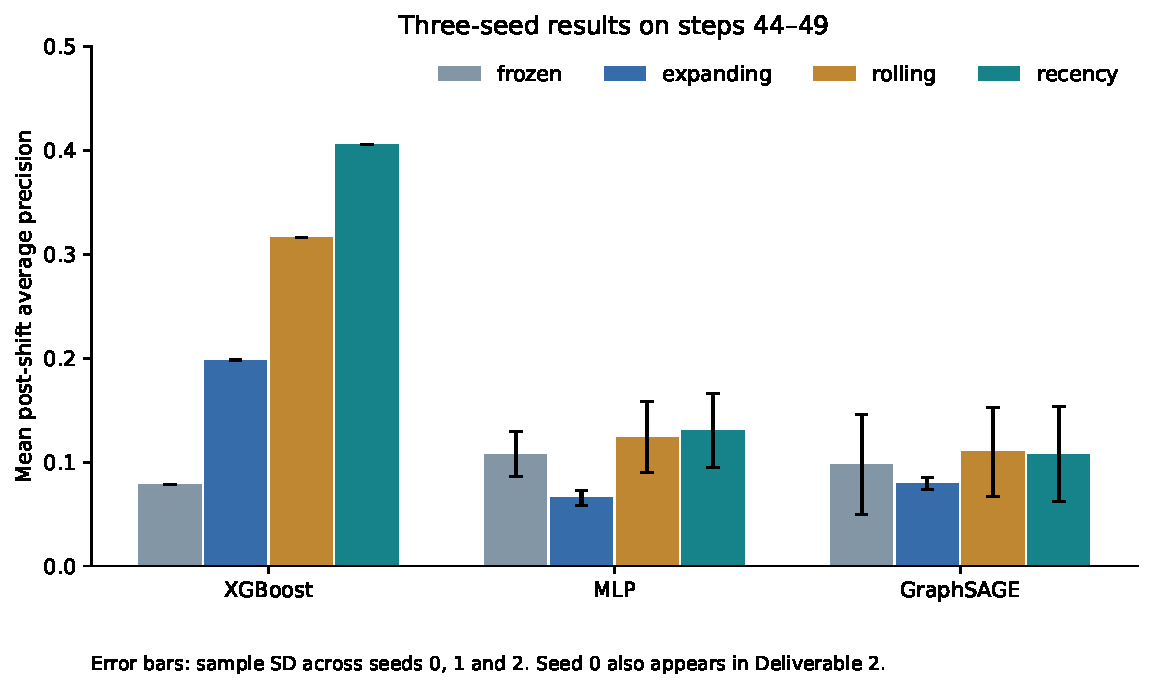
\includegraphics[width=0.88\textwidth]{three_seed_comparison.pdf}
\caption{All four adaptation policies across three seeds. Error bars show sample SD across seeds, not confidence intervals. Seed 0 appears in both deliverables. Identical XGBoost runs do not imply zero future-data uncertainty.}\label{fig:results}\end{figure*}

XGBoost with recency remains strongest at mean post-shift AP 0.4053 (Table~\ref{tab:main}). Its expanding and rolling values are 0.1983 and 0.3164. MLP's recency mean is 0.1303, compared with 0.0656 for expanding and 0.1239 for rolling. GraphSAGE's recency mean is 0.1077, compared with 0.0793 for expanding and 0.1100 for rolling. Thus recency is not the best mean policy for every family, and the graph model does not win the primary comparison. Figure~\ref{fig:results} retains all policies rather than selecting favorable runs.

Within-seed recency-minus-expanding AP gains average $0.2070\pm0.0000$ for XGBoost, $0.0647\pm0.0296$ for MLP, and $0.0284\pm0.0403$ for GraphSAGE. These descriptive contrasts suggest that recent-history emphasis benefits the evaluated tree configuration more consistently. They do not establish a universal architecture ranking or statistical significance. Neural parameter counts, optimization and selected budgets differ.

The XGBoost results are identical across the selected seeds under full-row/full-feature settings. This limits what its zero seed SD establishes. The neural means differ from the original seed-0 values because additional runs change the estimate, not because a newly tuned algorithm improves on Deliverable 2. No favorable seed replaces the original baseline, and no holdout-driven parameter search is introduced.

\subsection{Recovery and Degree-Based Diagnostics}
Sustained recovery requires two consecutive post-event snapshots with F1 at least 90\% of that combination's mean pre-event F1, each containing at least ten illicit and ten licit targets. Only pairs 47--48 and 48--49 meet the support condition. Recovery is not observed by 49 for any of the 36 combinations. A final-step rebound cannot satisfy a two-step rule without sufficient follow-up.

The new diagnostic stratifies known-label predictions by incoming degree computed from the original graph. It never uses neighbor labels as predictors and changes no features or thresholds. Zero incoming degree does not necessarily mean isolation because outgoing edges may exist. Diagnostic AP pools transactions within each phase/degree group before summarizing seeds; it differs from the snapshot-macro AP above.

\begin{table}[t]\caption{Post-shift recency diagnostic: mean pooled AP across seeds.}\centering\footnotesize\setlength{\tabcolsep}{3pt}
\begin{tabular}{lrrrrr}\toprule
Incoming & Known & Illicit & XGB & MLP & SAGE\\\midrule
0 & 2,109 & 116 & .5869 & .1429 & .1217\\
1 & 2,437 & 14 & .1986 & .0428 & .0266\\
2+ & 771 & 15 & .4199 & .0940 & .0834\\\bottomrule
\end{tabular}\label{tab:degree}\end{table}

The degree-map joins and all 216 diagnostic metric rows are recomputed successfully. GraphSAGE shows no consistent mean advantage in these strata (Table~\ref{tab:degree}). However, the connected groups contain only 14 and 15 illicit targets, and class prevalence differs markedly. These small retrospective subgroups cannot establish a causal graph effect. The result motivates careful error inspection rather than a new feature or threshold selected from test labels.

\subsection{Latency and Refinement Reflection}
A paired benchmark uses the same XGBoost/recency/seed-0/step-49/10\% workload in one Colab Python 3.13.16 process. It verifies equal metrics and queue IDs, performs three warmups per version, and alternates execution order over 30 measurements per version. Table~\ref{tab:latency} reports the saved runtime evidence.

\begin{table}[t]\caption{Colab warm Python callback latency, milliseconds.}\centering\small
\begin{tabular}{lrr}\toprule
Version & Median & 95th percentile\\\midrule
Deliverable 2 & 55.19 & 64.01\\
Deliverable 3 & 18.60 & 21.57\\\bottomrule
\end{tabular}\label{tab:latency}\end{table}

The median falls by about 66.3\%, a 2.97-fold speedup. This is a measured implementation improvement from avoiding repeated reads and work, not a training-speed or browser-latency claim. It excludes HTTP, network, startup, and human interaction; hardware load and cache state can change the result. A separate local measurement is retained without mixing its values with the Colab comparison.

The main lesson is that refinement need not force a higher predictive score. More complete evaluation exposes seed sensitivity and unsuccessful recovery, while validated inputs, explicit metric definitions, and faster replay make the same models easier to inspect. Before Deliverable 4, priorities are a recorded browser task walkthrough, clearer presentation of remaining uncertainty, and final report/demo consistency. Additional model complexity is optional and should not replace these checks.

\section{Responsible AI Reflection}
Illicit labels reflect what investigators detected and attributed. They can encode investigative priorities and blind spots, while unknown transactions can contain undetected illicit behavior. Evaluation on known targets therefore does not establish comprehensive laundering detection. Anonymized features do not support demographic fairness claims, and degree-group analysis is a structural diagnostic rather than a fairness audit.

False positives can harm legitimate users. Scores support human review only and must never trigger automatic sanctions, account closure, or legal accusations. The interface distinguishes observed labels, threshold decisions, and budget rankings. It states that weighted-model scores are uncalibrated. A low example score is not proof of legitimacy, and its selected observed label is not a representative evaluation sample.

CSV validation reduces silent feature-order and missing-value errors. The application does not write uploaded features to disk, although hosting providers may retain request logs. Credentials and raw source CSVs remain excluded from the distributed project. Small networks, bounded searches, reused artifacts and measured callback performance limit avoidable computation; no energy or carbon estimate is inferred from latency.

Transparency includes the unfavorable graph results, the absence of sustained recovery, selective labels, simulated label delay, and the reuse of the same test snapshots across seeds. AI tools assisted with design, code, analysis and documentation. Executed Colab training outputs, audits, verification JSON, and genuine screenshots support the reported progress. Independent user feedback and universal deployment reliability remain unclaimed.

\begin{thebibliography}{9}
\bibitem{elliptic} M. Weber et al., ``Anti-Money Laundering in Bitcoin: Experimenting with Graph Convolutional Networks for Financial Forensics,'' KDD Workshop on Anomaly Detection in Finance, 2019, arXiv:1908.02591.
\bibitem{xgboost} T. Chen and C. Guestrin, ``XGBoost: A Scalable Tree Boosting System,'' Proc. ACM SIGKDD, 2016, pp. 785--794.
\bibitem{sage} W. L. Hamilton, R. Ying, and J. Leskovec, ``Inductive Representation Learning on Large Graphs,'' Advances in Neural Information Processing Systems, 2017, arXiv:1706.02216.
\end{thebibliography}
\end{document}
